\section{Perancangan Perangkat Lunak}
\label{sec:perancangan-perangkat-lunak}

Pengujian hasil akurasi akselerator perangkat keras untuk \ac{RL} perlu diuji menggunakan sebuah kasus permasalahan \ac{RL}. Pada penelitian tugas akhir ini, kasus permasalahan yang dipilih adalah \ac{RL} untuk memecahkan permasalahan labirin \parencite{mini2023understanding}. Permasalahan labirin merupakan permasalahan dimana sebuah agent \ac{RL} diletakkan pada sebuah konfigurasi labirin yang diskrit yang telah dijelaskan pada sub sub-bab \ref{sub:sub-rl} dengan ilustrasi Gambar \ref{fig:ilustrasi-RL}. Rangkaian pengujian tersebut, agar dapat diujikan kepada akselerator perangkat keras, memerlukan tiga komponen untuk diimplementasikan sebagai berikut.

\vspace{-5mm}
\begin{enumerate}
	\begin{singlespace}
		\item \textit{Generator} konfigurasi labirin dengan input besar labirin (selanjutnya disebut sebagai dimensi labirin) yang dinamik.
		\item Algoritma yang mampu menjadi \textit{benchmark} akurasi dari hasil implementasi \ac{RL}.
		\item Algoritma dari pembelajaran agen \ac{RL} itu sendiri.
	\end{singlespace}
\end{enumerate}

Ketiga hal tersebut, akan dijelaskan secara sebagai pada sub sub-bab \ref{sec:sub-prim}, \ref{sec:sub-dfs}, dan \ref{sec:sub-pembelajaran-rl}.

\subsection{Algoritma Prim untuk \textit{Generator} Labirin}
\label{sec:sub-prim}

Skema labirin yang akan digunakan untuk melakukan pengujian implementasi \ac{RL} pada perangkat lunak dan perangkat keras akan dihasilkan dari algoritma Prim \parencite{devian2013implementasi}. Algoritma Prim dipilih karena dapat menghasilkan skema labirin yang dinamik berdasarkan masukan dimensi labirin, dengan entropi yang relatif konsisten. Implementasi detail dari algoritma Prim terdapat pada Algoritma \ref{alg:prim}.

\begin{algorithm}
	\makeatletter
	\renewcommand{\ALG@name}{Algoritma}
	\makeatother
	\caption{Prim \textit{Generator} Labirin}\label{alg:prim}
	\renewcommand{\algorithmicrequire}{\textbf{Masukan:}}
	\renewcommand{\algorithmicensure}{\textbf{Keluaran:}}
	\begin{algorithmic}[1]
		\Require $labirin$ dan $dimensi$
		\Ensure $labirin$ yang telah terbangun
		\State Inisialisasi $labirin$ penuh dengan halangan
		\State Buat halangan pertama jadi sel kosong
		\State Tambah semua halangan, disamping sel kosong, ke $list\_halangan$
		\While{$list\_halangan$ belum kosong}
		\State $halangan\_kini$ $\gets$ halangan acak di $list\_halangan$
		\If{$halangan\_kini$ hanya punya satu sel kosong didekatnya}
		\State Ubah $halangan\_kini$ menjadi sel kosong
		\State Masukkan halangan di sekitar $halangan\_kini$ ke $list\_halangan$
		\EndIf
		\State hapus $halangan\_kini$ dari $list\_halangan$
		\EndWhile
	\end{algorithmic}
\end{algorithm}

Algoritma \ref{alg:prim}, dapat diilustrasikan sesuai dengan Gambar \ref{fig:prim-visual}.

\begin{figure}[H]
	\centering
	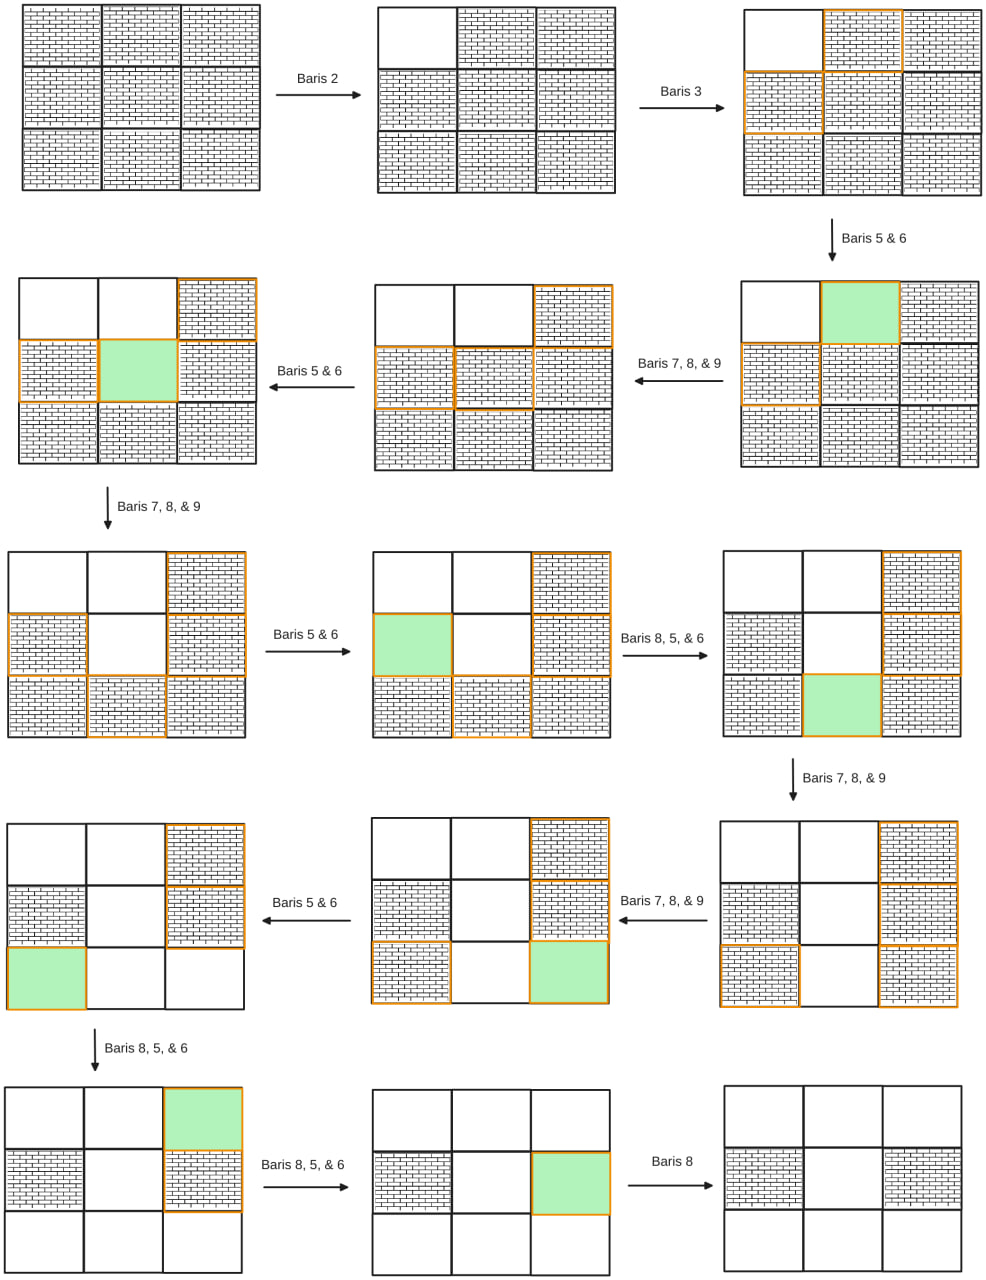
\includegraphics[width=1\textwidth]{chapter-3/prim-visual.jpg}
	\caption{Visualisasi Algoritma Prim}
	\label{fig:prim-visual}
\end{figure}

Pada Gambar \ref{fig:prim-visual}, halangan berkotak oranye merupakan halangan yang masuk kepada \textit{list\_halangan}dan halangan yang berkotak oranye dengan tengah hijau merupakan \textit{halangan\_kini} pada Algoritma \ref{alg:prim}. Keacakan pada algoritma Prim akan dikontrol untuk pengujian, sehingga dapat menghasilkan konfigurasi labirin yang sama berkali-kali untuk masukan dimensi labirin yang sama.

\subsection{Algoritma \ac{DFS} untuk \textit{Benchmark} Hasil \acl{RL}}
\label{sec:sub-dfs}

\acf{DFS} merupakan algoritma yang digunakan untuk memecahkan banyak permasalahan yang berhubungan dengan data struktur \textit{graph}. Algoritma ini pertama kali dipopulerkan oleh J. Hopcroft dan R. Tarjan pada \parencite{hopcroft1973algorithm} dengan ilustrasi diagram alir algoritma pada Gambar \ref{fig:hopcroft-dfs}.

\begin{figure}[H]
	\centering
	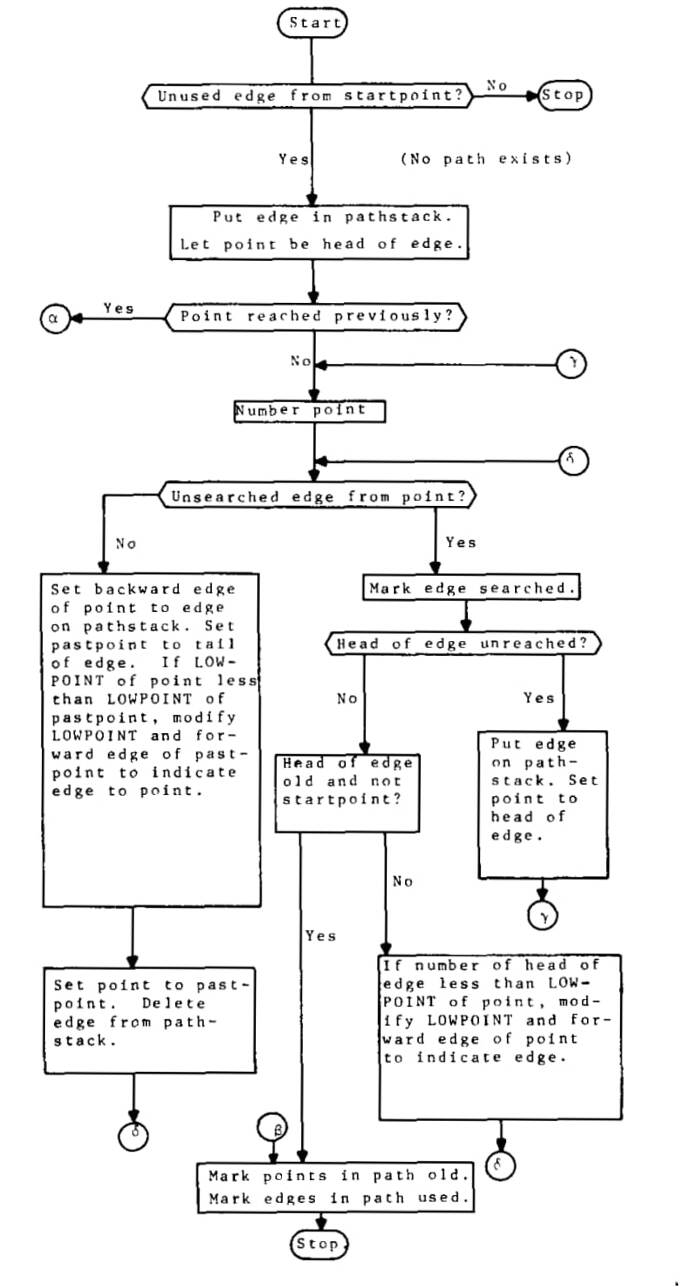
\includegraphics[width=0.7\textwidth]{chapter-3/path-finding-hopcroft.jpeg}
	\caption{Algoritma \ac{DFS} untuk \textit{Pathfinding} \parencite{hopcroft1973algorithm}}
	\label{fig:hopcroft-dfs}
\end{figure}

Pada penelitian ini, algoritma dari Gambar \ref{fig:hopcroft-dfs} disesuaikan dengan konteks permasalahan labirin. Hasil dari penyesuaian yang dilakukan dijelaskan secara detail pada Algoritma \ref{alg:dfs-sw}.

\begin{algorithm}
	\makeatletter
	\renewcommand{\ALG@name}{Algoritma}
	\makeatother
	\caption{\ac{DFS} Pada Labirin}\label{alg:dfs-sw}
	\renewcommand{\algorithmicrequire}{\textbf{Masukan:}}
	\renewcommand{\algorithmicensure}{\textbf{Keluaran:}}
	\begin{algorithmic}[1]
		\Require $baris$, $kolom$, dan $memori$
		\Ensure $langkah\_diambil$
		\State $memori \gets$ [$baris$,$kolom$]
		\If{[$baris$,$kolom$] = tujuan}
		\State return 0 \EndIf
		\State $langkah\_diambil$ $\gets$ NULL
		\For{$aksi$ dari [$gerak\_atas$, $gerak\_bawah$, $gerak\_kiri$, $gerak\_kanan$]}
		\State $kolom\_baru$, $baris\_baru$ $\gets$ lingkungan($aksi$, $kolom$, $baris$)
		\If{[$kolom\_baru$,$baris\_baru$] \textbf{tidak di} $memori$}
		\State $langkah\_DFS$ $\gets$ DFS($kolom\_baru$, $baris\_baru$, $memori$) + 1
		\If{$langkah\_diambil$ = NULL \textbf{or} $langkah\_diambil < langkah\_DFS$}
		\State $langkah\_diambil \gets langkah\_DFS$
		\EndIf
		\EndIf
		\EndFor
		\State return $langkah\_diambil$
	\end{algorithmic}
\end{algorithm}

Algoritma \ref{alg:dfs-sw} dapat divisualisasikan cara kerjanya sesuai dengan Gambar \ref{fig:dfs-visualization}.

\begin{figure}[H]
	\centering
	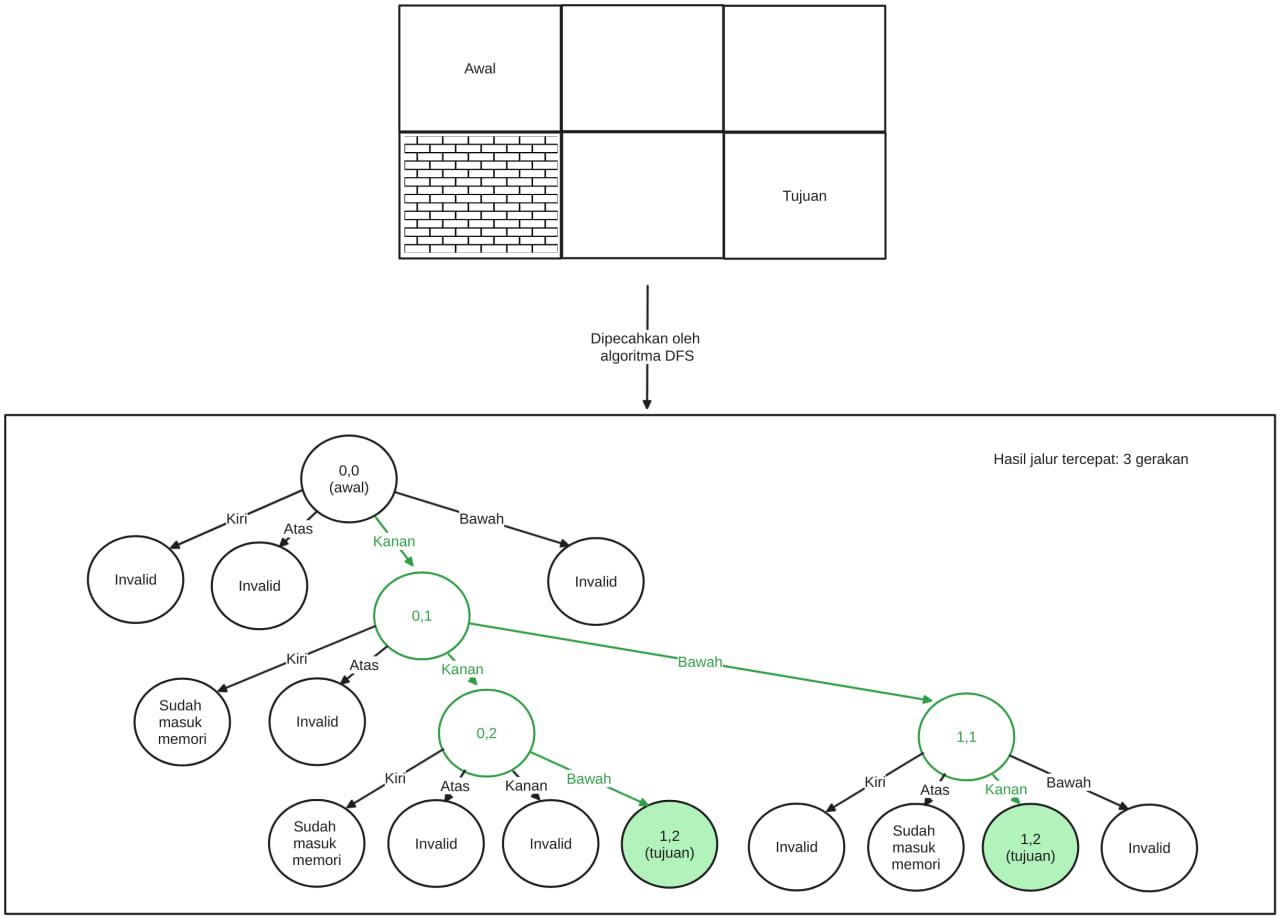
\includegraphics[width=1\textwidth]{chapter-3/dfs-tree.jpg}
	\caption{Visualisasi Algoritma \ac{DFS}}
	\label{fig:dfs-visualization}
\end{figure}

Pada Gambar \ref{fig:dfs-visualization}, lingkaran merupakan analogi pemanggilan fungsi \ac{DFS} pada Algoritma \ref{alg:dfs-sw} dengan teks didalamnya merupakan representasi input dari fungsi \ac{DFS} yaitu baris dan kolom. Garis hijau merupakan penanda jalur tercepat yang dihasilkan oleh DFS yang bisa diambil untuk memecahkan permasalahan labirin yang ada pada ilustrasi Gambar \ref{fig:dfs-visualization}. Hasil dari algoritma ini, akan digunakan untuk melakukan \textit{benchmark} dari pengujian algoritma \ac{RL} yang akan dibahas secara detail pada sub sub-bab \ref{sec:sub-pembelajaran-rl}.

\subsection{Algoritma Pembelajaran \acl{RL}}
\label{sec:sub-pembelajaran-rl}

Algoritma pembelajaran \ac{RL} yang digunakan pada penelitian ini diadopsi dari pembelajaran \ac{RL} menggunakan \textit{Q-Learning} dari penelitian \parencite{sutisna2023faraneq} yang dideskripsikan pada Algoritma \ref{alg:rl-qlearning}.

\begin{algorithm}
	\makeatletter
	\renewcommand{\ALG@name}{Algoritma}
	\makeatother
	\caption{\ac{RL} Menggunakan \textit{Q-Learning} Diadaptasi dari \parencite{sutisna2023faraneq}}\label{alg:rl-qlearning}
	\renewcommand{\algorithmicrequire}{\textbf{Masukan:}}
	\renewcommand{\algorithmicensure}{\textbf{Keluaran:}}
	\begin{algorithmic}[1]
		\Require jumlah episode, \textit{learning rate ($\alpha$)}, dan \textit{discount factor ($\gamma$)}
		\Ensure \textit{Q-Table}
		\State Inisialisasi \textit{Q-Table} untuk setiap \textit{state} dan aksi
		\While{$banyak\_episode < jumlah\_episode$}
		\State $s_{t} \gets s_0$
		\While{$s_t \neq s_{terminal}$}
		\State Pilih aksi ($A$) untuk \textit{state} kini ($s_t$)
		\State Lakukan $A$, dapatkan \textit{reward} dan $s_{t+1}$ \label{algline:q-reward}
		\State Hitung nilai Q-Table indeks terkini \Comment{dengan Persamaan \ref{eq:q-learning}}
		\State $s_t \gets s_{t+1}$
		\EndWhile
		\State $banyak\_episode \gets banyak\_episode + 1$
		\EndWhile
	\end{algorithmic}
\end{algorithm}

Fungsi \textit{reward} yang menghasilkan dari Algoritma \ref{alg:rl-qlearning} pada baris \ref{algline:q-reward} pada penelitian ini didesain sebagai fungsi skalar yang didesain secara iteratif, cara umum untuk mendesain fungsi \textit{reward} berdasarkan \parencite{hayes2022practical} pada agen \ac{RL}. Detail dari implementasi fungsi \textit{reward} pada penelitian ini terangkum pada Algoritma \ref{alg:rl-reward-function}.

\begin{algorithm}
	\makeatletter
	\renewcommand{\ALG@name}{Algoritma}
	\makeatother
	\caption{Desain Fungsi \textit{Reward}}\label{alg:rl-reward-function}
	\renewcommand{\algorithmicrequire}{\textbf{Masukan:}}
	\renewcommand{\algorithmicensure}{\textbf{Keluaran:}}
	\begin{algorithmic}[1]
		\Require $baris$, $kolom$, $memori$, dan aksi
		\Ensure $reward$
		\State $kolom\_baru$, $baris\_baru$ $\gets$ lingkungan($aksi$, $kolom$, $baris$)
		\If{[$kolom\_baru$,$baris$] = halangan} \label{algline:reward-c1}
		\State return $C_1$
		\EndIf
		\If{[$kolom\_baru$,$baris$] \textbf{ada di} $memori$} \label{algline:reward-c2}
		\State return $C_2$
		\EndIf
		\If{[$kolom\_baru$,$baris$] = tujuan} \label{algline:reward-c3}
		\State return $C_3$
		\EndIf
		\State return $C_4$ \label{algline:reward-c4}
	\end{algorithmic}
\end{algorithm}

Pada Algoritma \ref{alg:rl-reward-function} baris \ref{algline:reward-c1}, reward yang diberikan ($C_1$) akan berupa $punishment$, atau $reward$ yang bernilai negatif, yang digunakan untuk menghentikan agen dari melakukan pergerakan menuju halangan. Lalu, $punishment$ lain berada pada baris \ref{algline:reward-c2} ($C_2$) yang berupa $punishment$ untuk menghentikan agen bergerak ke sel kosong yang pernah dilalui sebelumnya. Satu-satunya $reward$ positif yang didapatkan berada pada baris \ref{algline:reward-c3} ($C_3$) yang digunakan untuk memastikan bahwa agen selalu menuju tujuan, menghindari efek $C_4$. Sedangkan $C_4$, pada baris \ref{algline:reward-c4}, merupakan $punishment$ yang digunakan untuk memastikan agen selalu mengambil jalut tercepat.

Algoritma \ref{alg:rl-reward-function} memiliki kekurangan ketidakstabilan untuk menghasilkan strategi optimal ($\pi^*$) dari permasalahan labirin ini. Hal ini, merupakan hal yang sering terjadi pada desain fungsi $reward$ untuk kasus pemilihan aksi diskrit. Salah satu contoh kasus ketidakstabilan ini dapat dilihat dari hasil plot \textit{cumulative reward} pada Gambar \ref{fig:cumulative-reward-faraneq} dari \parencite{sutisna2023faraneq} yang juga menggunakan kasus permasalahan labirin sebagai $benchmark$ dari akselerator yang dikembangkan.

\begin{figure}[H]
	\centering
	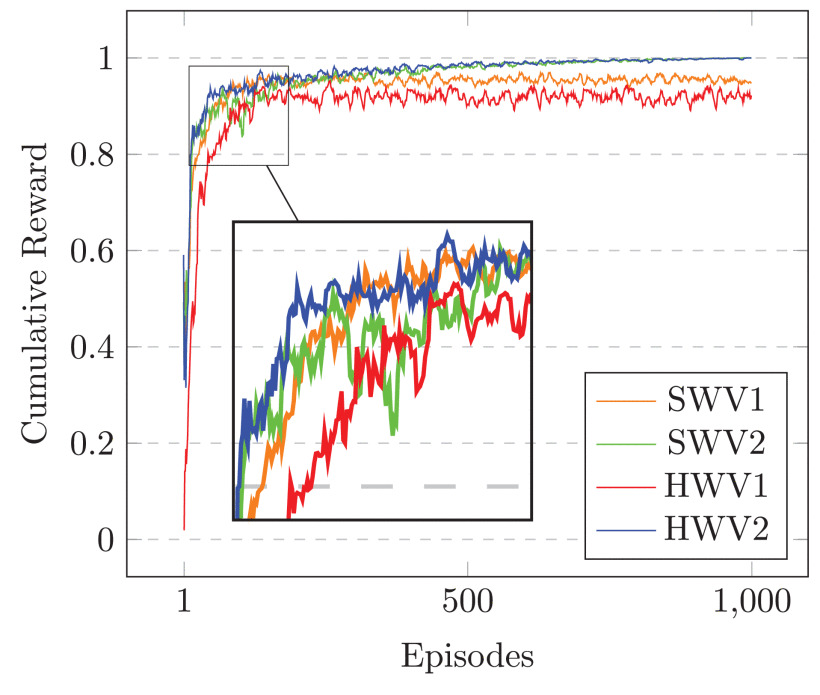
\includegraphics[width=0.8\textwidth]{chapter-3/faraneq-cumulative-rewards.jpg}
	\caption{Grafik \textit{Cumulative Reward} dari Penelitian \parencite{sutisna2023faraneq}}
	\label{fig:cumulative-reward-faraneq}
\end{figure}

Grafik \textit{cumulative reward} yang ditunjukkan pada Gambar \ref{fig:cumulative-reward-faraneq} memperlihatkan bahwa hasil \textit{cumulative reward} yang didapatkan dari pembelajaran \ac{RL} dari penelitian \parencite{sutisna2023faraneq} itu masih mengalami ketidakstabilan. Pada kasus lingkungan yang dimodelkan dengan fungsi \textit{reward} yang skalar dan diskrit, hal ini menjadi masalah karena turunnya grafik \textit{cumulative reward} adalah sebuah indikasi terjadinya pengambilan strategi/\textit{policy} yang tidak optimal setelah sebuah iterasi pembelajaran. Secara intrinsik, hal tersebut berarti algoritma pembelajaran tidak berhasil secara stabil menghasilkan strategi optimal atau $\pi^*$. Maka, Algoritma \ref{alg:rl-qlearning} diekstensi menggunakan metode memoisasi pintar yang diadopsi dari \parencite{mazaya2024reinforcement} yang dijelaskan pada Algoritma \ref{alg:rl-qmemo}.

\begin{algorithm}
	\makeatletter
	\renewcommand{\ALG@name}{Algoritma}
	\makeatother
	\caption{Ekstensi Algoritma \ac{RL} dengan Memoisasi Pintar Adopsi dari \parencite{mazaya2024reinforcement}}\label{alg:rl-qmemo}
	\renewcommand{\algorithmicrequire}{\textbf{Masukan:}}
	\renewcommand{\algorithmicensure}{\textbf{Keluaran:}}
	\begin{algorithmic}[1]
		\Require jumlah episode, \textit{learning rate} ($\alpha$), dan \textit{discount factor} ($\gamma$)
		\Ensure \textit{Q-Table}
		\State Inisialisasi \textit{Q-Table} untuk setiap \textit{state} dan aksi
		\While{$banyak\_episode < jumlah\_episode$}
		\State $s_{t} \gets s_0$
		\While{$s_t \neq s_{terminal}$}
		\State Pilih aksi ($A$) untuk \textit{state} kini ($s_t$)
		\State Lakukan $A$, dapatkan \textit{reward} dan $s_{t+1}$
		\State Hitung nilai Q-Table indeks terkini \Comment{dengan Persamaan \ref{eq:q-learning}}
		\State $s_t \gets s_{t+1}$
		\EndWhile
		\State $banyak\_episode \gets banyak\_episode + 1$
		\State $cr_t$ $\gets$ \textit{cumulative reward} dari \textit{Q-Table}
		\If{$cr_t\ >\ cr_{t-1}$}
		\State Ubah nilai $maxQ(s_{t+1},a))$ dari \textit{Q-Table} \label{algline:q-memo-equation} \Comment{dengan Persamaan \ref{eq:q-memo-overwrite}}
		\EndIf
		\State $cr_{t-1} \gets cr_t$
		\State \textit{memori Q-Table} $\gets$ \textit{Q-Table}
		\State $episode \gets episode + 1$
		\EndWhile
	\end{algorithmic}
\end{algorithm}

Inti dari ekstensi Algoritma \ref{alg:rl-qmemo} berada pada baris \ref{algline:q-memo-equation} yang melakukan perubahan nilai $maxQ(s_{t+1},a))$ dari \textit{Q-Table} menggunakan Persamaan .

\begin{equation}
	\label{eq:q-memo-overwrite}
	Q(s_{t},a_{t_x}) =	Q(s_{t},a_{t_y}) + \delta
\end{equation}

Pada Persamaan \ref{eq:q-memo-overwrite}, \(a_{t_x}\) adalah aksi yang memberikan nilai \textit{memori Q-Table} yang maksimal pada state $s_t$; \(a_{t_y}\) adalah aksi yang memberikan nilai \textit{Q-Table} yang maksimal pada state $s_t$; \(\delta\) adalah konstanta yang digunakan untuk membuat \(Q(s_{t},a_{t_x})\) di \textit{Q-Table} lebih besar dari \(Q(s_{t},a_{t_y})\) di \textit{memori Q-Table} sehingga menjadikan \(Q(s_{t},a_{t_x})\) nilai maksimal pada \textit{Q-Table}.

Implementasi dari ekstensi pada Algoritma \ref{alg:rl-qmemo} bertujuan untuk mendapatkan hasil \textit{Q-Table} yang memiliki $maxQ(s_{t+1},a))$, dari Persamaan \ref{eq:q-learning}, yang stabil tanpa menghilangkan nilai pembelajaran dari iterasi sebelumnya. Gambar \ref{fig:q-memo-ilustration}, memberikan ilustrasi bagaimana cara kerja Algoritma \ref{alg:rl-qmemo} secara detail.

\begin{figure}[H]
	\centering
	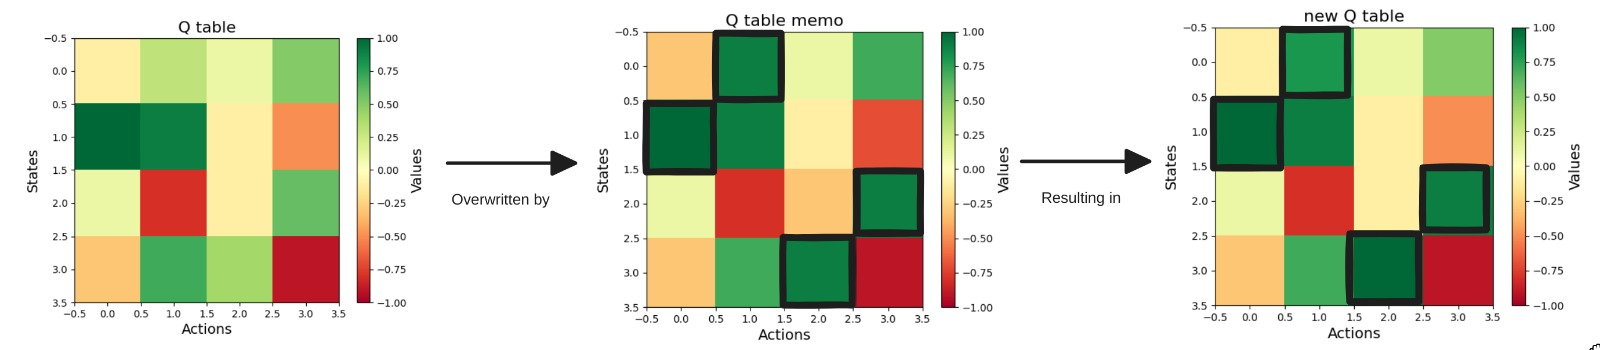
\includegraphics[width=1\textwidth]{chapter-3/q-memo-ilustration.jpg}
	\caption{Ilustrasi Algoritma \ref{alg:rl-qmemo} dari \parencite{mazaya2024reinforcement}}
	\label{fig:q-memo-ilustration}
\end{figure}

Pada Gambar \ref{fig:q-memo-ilustration}, diilustrasikan dua tahapan utama dari Persamaan \ref{eq:q-memo-overwrite}: pemilihan $a_{t_y}$ dan pengubahan nilai  $Q(s_{t},a_{t_x})$ dengan nilai $Q(s_{t},a_{t_y}) + \delta$. Terdapat tiga \textit{heatmap} pada Gambar \ref{fig:q-memo-ilustration}. Dari kiri ke kanan, \textit{heatmap} pertama merupakan ilustrasi dari sebuah nilai \textit{Q-Table} dari sebuah iterasi yang mengalami penurunan nilai \textit{cumulative reward}. \textit{Heatmap} kedua merupakan ilustrasi dari memori \textit{Q-Table} dari iterasi sebelumnya dengan nilai yang diberi kotak hitam adalah $Q(s_{t},a_{t_y})$. Lalu, \textit{heatmap} ketiga merupakan ilustrasi dari \textit{Q-Table} dari heatmap pertama yang nilai $Q(s_{t},a_{t_y})$-nya sudah diubah menjadi lebih tinggi daripada $Q(s_{t},a_{t_x})$.

Pengujian pembelajaran agen \ac{RL} menggunakan Algoritma \ref{alg:rl-qmemo} dilakukan dengan variasi dimensi labirin dan episode pembelajaran yang kemudian akan dibandingkan hasil performanya dengan implementasi pada akselerator perangkat keras.
